\documentclass{article}%
\usepackage[T1]{fontenc}%
\usepackage[utf8]{inputenc}%
\usepackage{lmodern}%
\usepackage{textcomp}%
\usepackage{lastpage}%
\usepackage{geometry}%
\geometry{left=3cm,right=3cm,bottom=2cm,top=1cm}%
\usepackage[russian]{babel}%
\usepackage{amsmath}%
\usepackage{amssymb}%
\usepackage{amsfonts}%
\usepackage{mathtext}%
\usepackage{graphicx}%
%
%
%
\begin{document}%
\normalsize%
\begin{center}%
\vspace*{\fill}%
{\LARGE\textbf{Лабораторная работа № 3.05: \\ Температурная зависимость электрического сопротивления металла и полупроводника}}\\[1cm]%
{\Large Исхаков Камиль Фархатович}\\[1cm]%
{\Large \today}%
\vspace*{\fill}%
\end{center}%
\newpage%
\section{Основные формулы}%
\label{sec:}%
Закон Ома для участка цепи:\begin{displaymath}R=\frac{U}{I}\end{displaymath}%
\newline%
где $R$ - сопротивление, $U$ - напряжение, $I$ -  сила ток\\%
Cопротивление полупроводника:\begin{displaymath}R_{\text{п}} = R_m\exp{(\frac{E_g}{2kT})}\end{displaymath}%
\newline%
где $kT$ - средняя энергия теплового движения, $R_m$ - предел к которому стремится значение сопротивления полупроводника при повышении температуры\\%
Формула для расчета ширины запрещенной зоны:\begin{displaymath}E_g=2k \cdot \frac{\Delta \ln({R_{\text{п}}})}{\Delta (1/T)}\end{displaymath}%
\newline%
где $k$ - постоянная Больцмана, $k=1,38*10^{-23} \textit{ Дж/К}=8,62*10^{-5}\textit{ эВ/К}$)\\%
Зависимость сопротивления от температуры для металла при небольших диапазонах температур:\begin{displaymath}R_{\text{м}} = R_0(1+\alpha T)\end{displaymath}%
\newline%
где $R_0$ - сопротивление данного образца при температуре $0^\circ C$, $\alpha$ - температурный коэффициент сопротивления\\

%
\section{Результаты эксперимента}%
\label{sec:}%


\begin{table}[h!]%
\centering%
\begin{tabular}{|c|c|c|c|c|c|}%
\hline%
$T$, К&$I$, мкА&$U$, В&$R$, Ом&$\ln{R}$&$\frac{10^3}{T}$, 1/К\\%
\hline%
305&1159&0.360&310.613&5.739&3.279\\%
\hline%
315&1258&0.256&203.498&5.316&3.175\\%
\hline%
325&1337&0.184&137.622&4.925&3.077\\%
\hline%
335&1387&0.128&92.286&4.525&2.985\\%
\hline%
345&1424&0.091&63.904&4.157&2.899\\%
\hline%
\end{tabular}%
\caption{Полупроводниковый образец}%
\end{table}

%


\begin{table}[h!]%
\centering%
\begin{tabular}{|c|c|c|c|c|}%
\hline%
$T$, К&$I$, мкА&$U$, В&$R$, кОм&$t$, °C\\%
\hline%
345&1098&1.496&1.362&72°\\%
\hline%
335&1113&1.468&1.319&62°\\%
\hline%
325&1125&1.439&1.279&52°\\%
\hline%
315&1146&1.412&1.232&42°\\%
\hline%
305&1164&1.384&1.189&32°\\%
\hline%
\end{tabular}%
\caption{Металлический образец образец}%
\end{table}

%


\begin{table}[h!]%
\centering%
\begin{tabular}{|c|c|c|}%
\hline%
$i$&$j$&$\alpha_{ij}$, $10^{-3}$ $\text{К}^{-1}$\\%
\hline%
1&3&3.903\\%
\hline%
2&4&4.146\\%
\hline%
3&5&4.306\\%
\hline%
\multicolumn{2}{|c|}{$\langle \alpha \rangle$}&4.118\\%
\hline%
\end{tabular}%
\caption{Температурный коэффициент сопротивления металла}%
\end{table}

%


\begin{table}[h!]%
\centering%
\begin{tabular}{|c|c|c|c|}%
\hline%
$i$&$j$&$E_{ij}$, Дж&$E_{ij}$, эВ\\%
\hline%
1&3&$0.111 \cdot 10^{-18}$&0.695\\%
\hline%
2&4&$0.115 \cdot 10^{-18}$&0.718\\%
\hline%
3&5&$0.119 \cdot 10^{-18}$&0.741\\%
\hline%
\multicolumn{2}{|c|}{$\langle E \rangle$}&$0.115 \cdot 10^{-18}$&0.718\\%
\hline%
\end{tabular}%
\caption{Ширина запрещенной зоны полупроводника}%
\end{table}

%
\newpage%


\begin{figure}[h!]%
\centering%
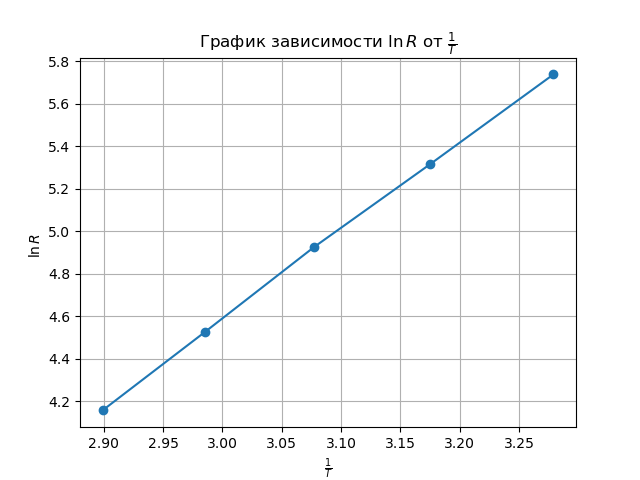
\includegraphics[width=300px]{LnR_vs_T.png}%
\caption{График зависимости $\ln{R}$ от $\frac{1}{T}$}%
\end{figure}

%


\begin{figure}[h!]%
\centering%
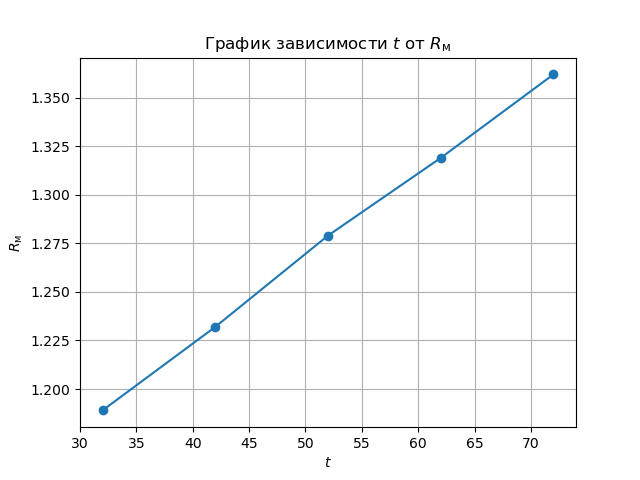
\includegraphics[width=300px]{kR_vs_t.png}%
\caption{График зависимости $t$ от $R_\text{м}$}%
\end{figure}

%
\section{Оценка погрешностей}%
\label{sec:}%
Для погрешности температурного коэффициента сопротивления используем формулу для стандартного отклонения среднего значения: \[ \Delta \alpha = t_{\alpha, n} \sqrt{\frac{\sum_{i=1}^n (\alpha_{ij} - \langle \alpha \rangle)^2}{n(n-1)}}\]%
\\ Вычисленная погрешность ($\Delta \alpha$): $0.25 \cdot 10^{-3}$ $\frac{1}{^\circ C}$%
\\Для погрешности ширины запрещенной зоны используем формулу для стандартного отклонения среднего значения:\[ \Delta E_g = t_{\alpha, n} \sqrt{\frac{\sum_{i=1}^n (E_{gij} - \langle E_g \rangle)^2}{n(n-1)}}\]%
\\ Вычисленная абсолютная погрешность ($\Delta E_g$): $0.452 \cdot 10^{-20}$ Дж%
\\ Вычисленная абсолютная погрешность ($\Delta E_g$): 0.028 эВ

%
\section{Выводы}%
\label{sec:}%
Табличное значение коэффициента сопротивления меди: $4,28 \cdot 10^{-3} \text{ К}^{-1}$\\%
Табличное значение ширины запрещенной зоны германия: $0,72 \text{ эВ}$\\%
Построенные графики имеют линейный вид, что согласуется с теоретическим поведением полупроводника и металла при нагревании. Исходя из полученного среднего значения  коэффициента сопротивления металла и абсолютной погрешности, можно сделать вывод,что наиболее вероятным металлическим образцом в данной лабораторной работе является медь. Аналогично, исходя из полученного среднего значения  ширины запрещенной зоны полупроводника и абсолютной погрешности, можно сделать вывод,что наиболее вероятным полупроводниковым образцом образцом в данной лабораторной работе является германий. Также в данной лабораторной работе подтвердились следующие теоретические выкладки – сопротивление металла при нагревании увеличивается, а у полупроводника наоборот – уменьшается.

%
\end{document}